% To produce pdf under linux, run
% pdflatex hw2.tex

% Credit for this template goes to Dr. Jerry Zhu.

\documentclass{article}
\usepackage[margin=1in]{geometry}
\usepackage{amsmath,amssymb}
\usepackage{bbm}
\usepackage{graphicx}
\usepackage{hyperref}
\usepackage{outlines}
\usepackage{enumitem}
\usepackage{float}
\usepackage{xcolor}
\usepackage{parskip}
\usepackage[skip=0.5\baselineskip]{caption}
\usepackage{subcaption}

\def\bfx{\mathbf x}
\def\R{\mathbb R}
\def\E{\mathbb E}
\def\argmax{\mathrm{argmax}}
\def\argmin{\mathrm{argmin}}


\newenvironment{soln}{
	\leavevmode\color{red}\ignorespaces
}{}



\title{CS760 Spring 2019 Homework 3}
\author{Due Mar 26 at 11:59pm}
\date{}
\begin{document}
\maketitle


%%%%%%%%%%%%%%%%%%%%%%%%%%%%%%%%%%%%%%%%%%%%%%%%%%%%%%%%%%%%%%%%%%%%%%%%%
% Insert your name and email here:

Name: Xinyi Li 

Email: xli646@wisc.edu

%%%%%%%%%%%%%%%%%%%%%%%%%%%%%%%%%%%%%%%%%%%%%%%%%%%%%%%%%%%%%%%%%%%%%%%%%


\section*{Written Problems}
\subsection*{Part3}
Datasets: magic\\
Learning rate: 0.01\\
Max num of epochs: 30\\
Number of hidden units: 10\\
\begin{figure}[h!]
  \centering
  \begin{subfigure}[b]{0.45\linewidth}
    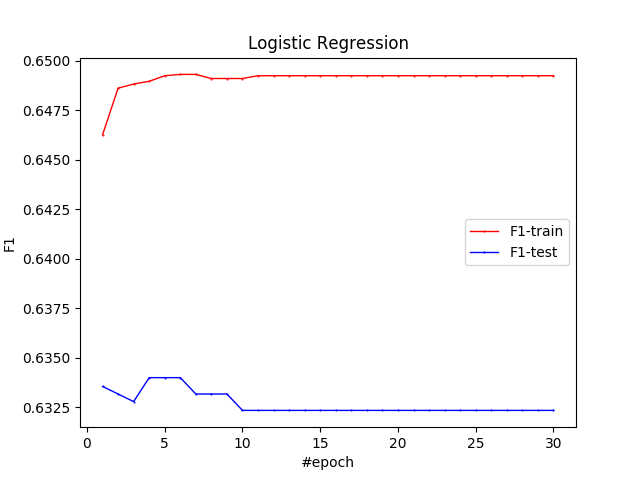
\includegraphics[width=\linewidth]{logistic_F1.png}
    \caption{}
  \end{subfigure}
  \begin{subfigure}[b]{0.45\linewidth}
    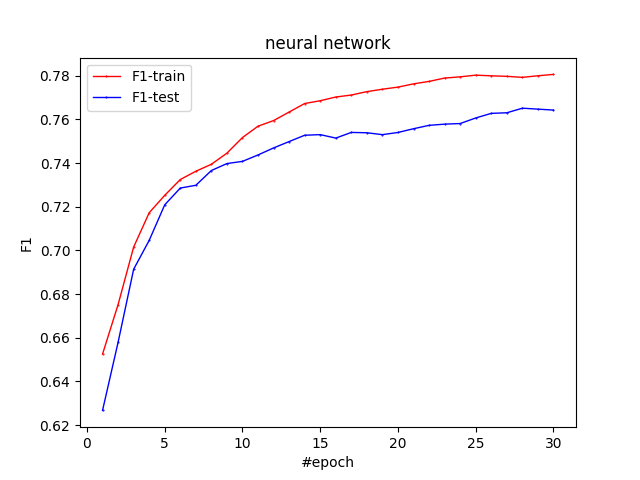
\includegraphics[width=\linewidth]{nnet_F1.png}
    \caption{}
      \end{subfigure}
  \caption{(a) F1 scores for logistic regression (b) F1 scores for neural network.} 
  \label{lj}
 \end{figure}

For logistic regression, F1-score for training data increases with number of epochs increases. However, F1-score for test data decreases. This indicates that overfitting occurs for logistic regression.\\
For neural network, F1-scores for both training and test data increase as number of epochs increases. Overfitting doesn't happen for neural network.\\
Unless the number of epochs is very small, neural network outperforms logistic regression.


\end{document}
